\chapter{Electromagnetic Shower Energy Reconstruction in SBND}
\label{chap:Energy_Reco}
\section{Motivation for Improving the Shower Energy Reconstruction}

Important for the selections - directly used as one of the cuts. 
EM showers is the driving factor in obtaining Enu reco.


\section{Event Production and Reconstruction in LArSoft}\label{sec:Event Production and Reconstruction in LArSoft}

Use vertex sample - make life easier for Pandora.

\gls{mc} event production and analysis is performed using the \gls{larsoft} framework which interfaces with a number of other frameworks such as \gls{genie} for event generation, \gls{geant4} for event simulation and Pandora for event reconstruction. \gls{larsoft} has been designed to work for many liquid argon based neutrino experiments including \gls{sbn} with many of the underlying algorithms being common to all experiments \cite{larsoft}\cite{larsoft_paper}.

Reconstructed quantities are the main focus of this section and these are typically derived from the reconstructed charge which is obtained in the following steps;
\begin{itemize}
    \item Drifting electrons induce current on a wire.
    \item Extract the signal on the wire from the E-field and any noise. 
    \item A hit finding algorithm identifies any significant waveforms and classifies these as hits across a certain time window (number of ticks). 
    \item The Pandora pattern recognition software clusters the hits together such that they represent an individual particle. This is initially done in 2D, followed by matching the clusters between the wire planes in order to produce 3D clusters.
    \item The lineage of the particles is identified and the particles are classified as either track or shower like.
\end{itemize}

A number of different hit finding algorithms exist, but the default one used by \gls{larsoft} is the \textit{GausHitFinder}. Once the algorithm has identified a waveform that peaks above some threshold (the threshold in \gls{sbnd} is 10 \gls{adc} counts), it attempts to fit one or more Gaussians to the waveform. For each peak, the centre and width are identified and these values are used to produce the associated Gaussian fit. For most cases the GausHitFinder works well, but two areas where it can struggle are resolving hits which are closely spaced and fitting a Gaussian to waveforms that are not well represented by a Gaussian. The latter tends to occur when charge is directed towards the wire planes (e.g. from a shower that was produced at a large angle to the beam line instead of being mostly forward going) which causes a long pulse train on but a few wires. This results in long waveforms where the \gls{adc} count is above threshold for many ticks and is without a clear central peak. These long waveforms may be better represented by a series of N-Gaussians, however, this is still far from perfect and fitting a large number of peaks can appreciably increase computing time \cite{gaushitfinder}. 

\section{Overview of Shower Energy Reconstruction in SBND}\label{subchap:shower reco overview}

Currently, there are three algorithms available for reconstructing \gls{em} shower energy within \gls{sbnd} as part of the \textit{LArPandoraShower} suite of tools, each of which are described below. Regardless of the algorithm used, the initial approach is the same for all three methods which is as follows,
\begin{enumerate}
    \item Identify the hits associated with a given wire plane.
    \item Integrate the hits to obtain the associated charge in \gls{adc} units whilst correcting for electron lifetime. 
    \item Convert the charge in \gls{adc} units to a conventional charge (number of electrons) using the calibration constant which is part of the calorimetry algorithm (This step was not performed in the case of the \textit{Linear Energy tool}). 
\end{enumerate}

Once the charge of a hit has been determined, the final steps which involve converting the charge to energy becomes method dependent. The other major detector effect that still needs to be considered is recombination, which is modelled by the Modified Box Recombination Model and given by  
\begin{equation}\label{eqn:ModBox}
    \frac{dE}{dx} = \frac{\exp{(\frac{\beta}{\rho \mathcal{E}} W_{ion}.\frac{dQ}{dx}}) - \alpha}{\frac{\beta}{\rho \mathcal{E}}},
\end{equation}
where $\frac{dE}{dx}$ is the deposited energy per unit length, $\frac{dQ}{dx}$ is the deposited charge per unit length,  $\mathcal{E}$ is the electric field in the detector, $\rho$ is the density of liquid argon, $W_{ion} = 23.6$ eV which is the energy required to ionise an argon atom, $\alpha = 0.93 \pm 0.02$ and $\beta = 0.212 \pm 0.002$ (kV/cm)(g/cm$^2$)/MeV. The values for parameters $\alpha$ and $\beta$ are results from the \Gls{argoneut} experiment \cite{ArgoNeuT_recombination_paper}. The recombination correction, \textit{R}, is given by $\frac{\frac{dQ}{dx}.W_{ion}}{\frac{dE}{dx}}$.


Since the recombination model is $\frac{dE}{dx}$ dependent, an accurate path length \textit{dx} is needed which requires 3D reconstruction of the direction. Doing this for a shower which is inherently \textit{messy} is not straightforward and unlike the electron lifetime it is therefore difficult to directly correct for the recombination effect \cite{MicroBooNE_photon_Ereco_paper}. Two different approaches have been considered and are discussed in the relevant energy reconstruction methods below; 1) Assume a nominal recombination value for all hits and 2) use a lookup curve which relates the collected charge to energy which circumvents the need to evaluate a recombination correction directly because it already gets accounted for in the curve.

In the analysis and validation of the shower reconstruction, a number of \textit{true} and \textit{reco} quantities are considered. Care must be taken that it is clear what each value relates to. For clarity, the following quantities are explicitly described;
\begin{itemize}
    \item Collected charge (or energy): This is the charge that is seen by the wire planes. 
    \item Deposited charge (or energy): This is the charge that is initially deposited in the detector. Typically this would be obtained from the collected charge by correcting for the electron lifetime and the recombination effect.
    \item Hit energy: This is the energy associated with each individual hit. Both true and reco values may be obtained.
    \item Energy of showering particle: This is the energy of the particle which results in the shower which is being investigated. 
\end{itemize}
\subsection{Linear Energy Tool}\label{subchap:Linear Energy Tool}
The first shower energy reconstruction method developed was the \textit{Shower Linear Energy tool}. This tool relies on the linear relationship between the true energy deposited in the detector and the reconstructed charge from \gls{mip} muons. A sample of \Gls{mc} muons are used as calibration because the $\frac{dE}{dx}$ value for electrons and \Gls{mip} muons are not dissimilar. The relationship between the charge obtained from the hits due to the muons and the energy deposited by the muons is shown in \FigureRef{fig:linear lookup curve}. A linear relationship such as this is comparable to assuming a constant recombination factor. 



%\begin{center}
%    \centering
%    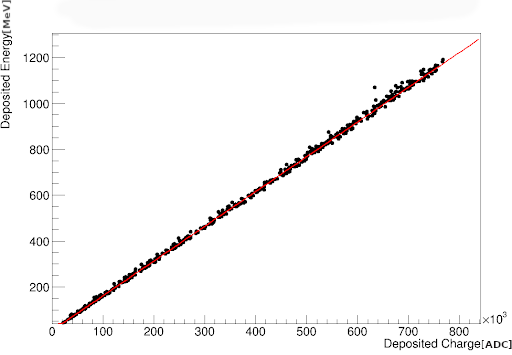
\includegraphics[width = 0.7\textwidth]{figures-chap4/linear_energy_lookup_curve1.png}
%    \captionsetup{type=figure}
%    \captionof{figure}{The linear relationship between deposited charge and energy. Produced from a sample of muons used for calibrating the \textit{Shower Linear Energy tool.}}
%    \label{fig:linear lookup curve}
%\end{center}
\newpage
\begin{figure}[h]
    \centering
    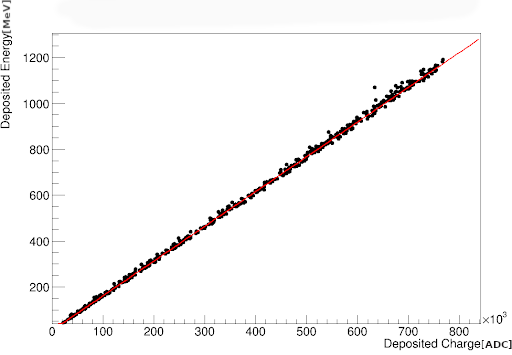
\includegraphics[width = \largefigwidth]{figures-chap4/linear_energy_lookup_curve1.png}
    \caption{The linear relationship between deposited charge and energy. Produced from a sample of muons used for calibrating the \textit{Shower Linear Energy tool.}}
    \label{fig:linear lookup curve}
\end{figure}



To estimate the reconstructed shower energy, the charge found to be associated with a shower would be used to directly read off the associated energy from the linear calibration. A further recombination correction is not required as it has already been accounted for in the charge to energy conversion. The peformance of the \textit{Shower Linear Energy tool} is shown in \FigureRef{fig:linear_kGeVelectrons}, however, it has been largely disfavoured since the development of the two other reconstruction tools. 

\subsection{Number of Electrons to Energy}\label{subchap:kGeVToElectrons}
The \textit{Shower Num Electrons Energy tool} was developed to move away from being reliant on in-house calibration curves and instead use the pre-existing calibration available in the \Gls{sbnd} portion of the \Gls{larsoft} framework. This has the advantage of being much more flexible to physics changes. For example a change in the recombination correction could be investigated by changing a single number, whereas, for the \textit{Shower Linear Energy tool}, the calibration curves would have to be regenerated. The number of electrons are found from the \gls{adc} charge and are then directly converted to energy using a \textit{GeVToElectrons} scale factor which is the inverse of the energy required to ionise an argon atom. With this method a correction to account for recombination is still required. A nominal recombination value of 0.64 is used for all hits. 

The nominal recombination value was calculated by simulating electrons with a large (effectively infinite) lifetime and turning off any diffusion effects. The only thing remaining that may impact the collected energy is the recombination effect and therefore taking the ratio between the collected and deposited energy will give a value for the recombination value. For electrons, it was found that the recombination value was fairly constant at a value of 0.64 across a broad range of energies \cite{recombination_0.64}. 



\newpage


\begin{comment}

An attempt to correct for the \Gls{sce} can be made with this method by utilising the Modified Box Recombination Model which is given by \begin{equation}\label{eqn:ModBox}
    \frac{dE}{dx} = \frac{\exp{(\frac{\beta}{\rho \mathcal{E}} W_{ion}.\frac{dQ}{dx}}) - \alpha}{\frac{\beta}{\rho \mathcal{E}}}
\end{equation}
where $\frac{dE}{dx}$ is the deposited energy per unit length, $\frac{dQ}{dx}$ is the deposited charge per unit length,  $\mathcal{E}$ is the electric field in the detector, $\rho$ is the density of liquid argon, $W_{ion} = 23.6$ eV which is the energy required to ionise an argon atom, $\alpha = 0.93 \pm 0.02$ and $\beta = 0.212 \pm 0.002$ (kV/cm)(g/cm$^2$)/MeV. The values for parameters $\alpha$ and $\beta$ are results from the \Gls{argoneut} experiment \cite{ArgoNeuT_recombination_paper}. The recombination correction, \textit{R} is given by $\frac{\frac{dQ}{dx}.W_{ion}}{\frac{dE}{dx}}$ and by taking the nominal values of \textit{R} and $\mathcal{E}$ a nominal value for $\frac{dE}{dx}$ is calculated using \EquationRef{eqn:ModBox}. Assuming the nominal value of $\frac{dE}{dx}$ is constant, \textit{R} may be expressed as $R = R(\mathcal{E}$). For each of the hits, their corresponding \Gls{sp} are found and the coordinates of the \Gls{sp} in the detector are determined. Instead of using the nominal value for $\mathcal{E}$, the local value for $\mathcal{E}$ at the position of the \Gls{sp} is used and the corresponding value for \textit{R} is calculated. The method to estimate the reconstructed energy is the same as the case without any \Gls{sce} corrections except the modified value for \textit{R} is used. In the case that a hit has no corresponding \Gls{sp}, the charge weighted centre of the shower is found and the local value of $\mathcal{E}$ at this point is used instead.

\begin{figure}[h]
    \centering
    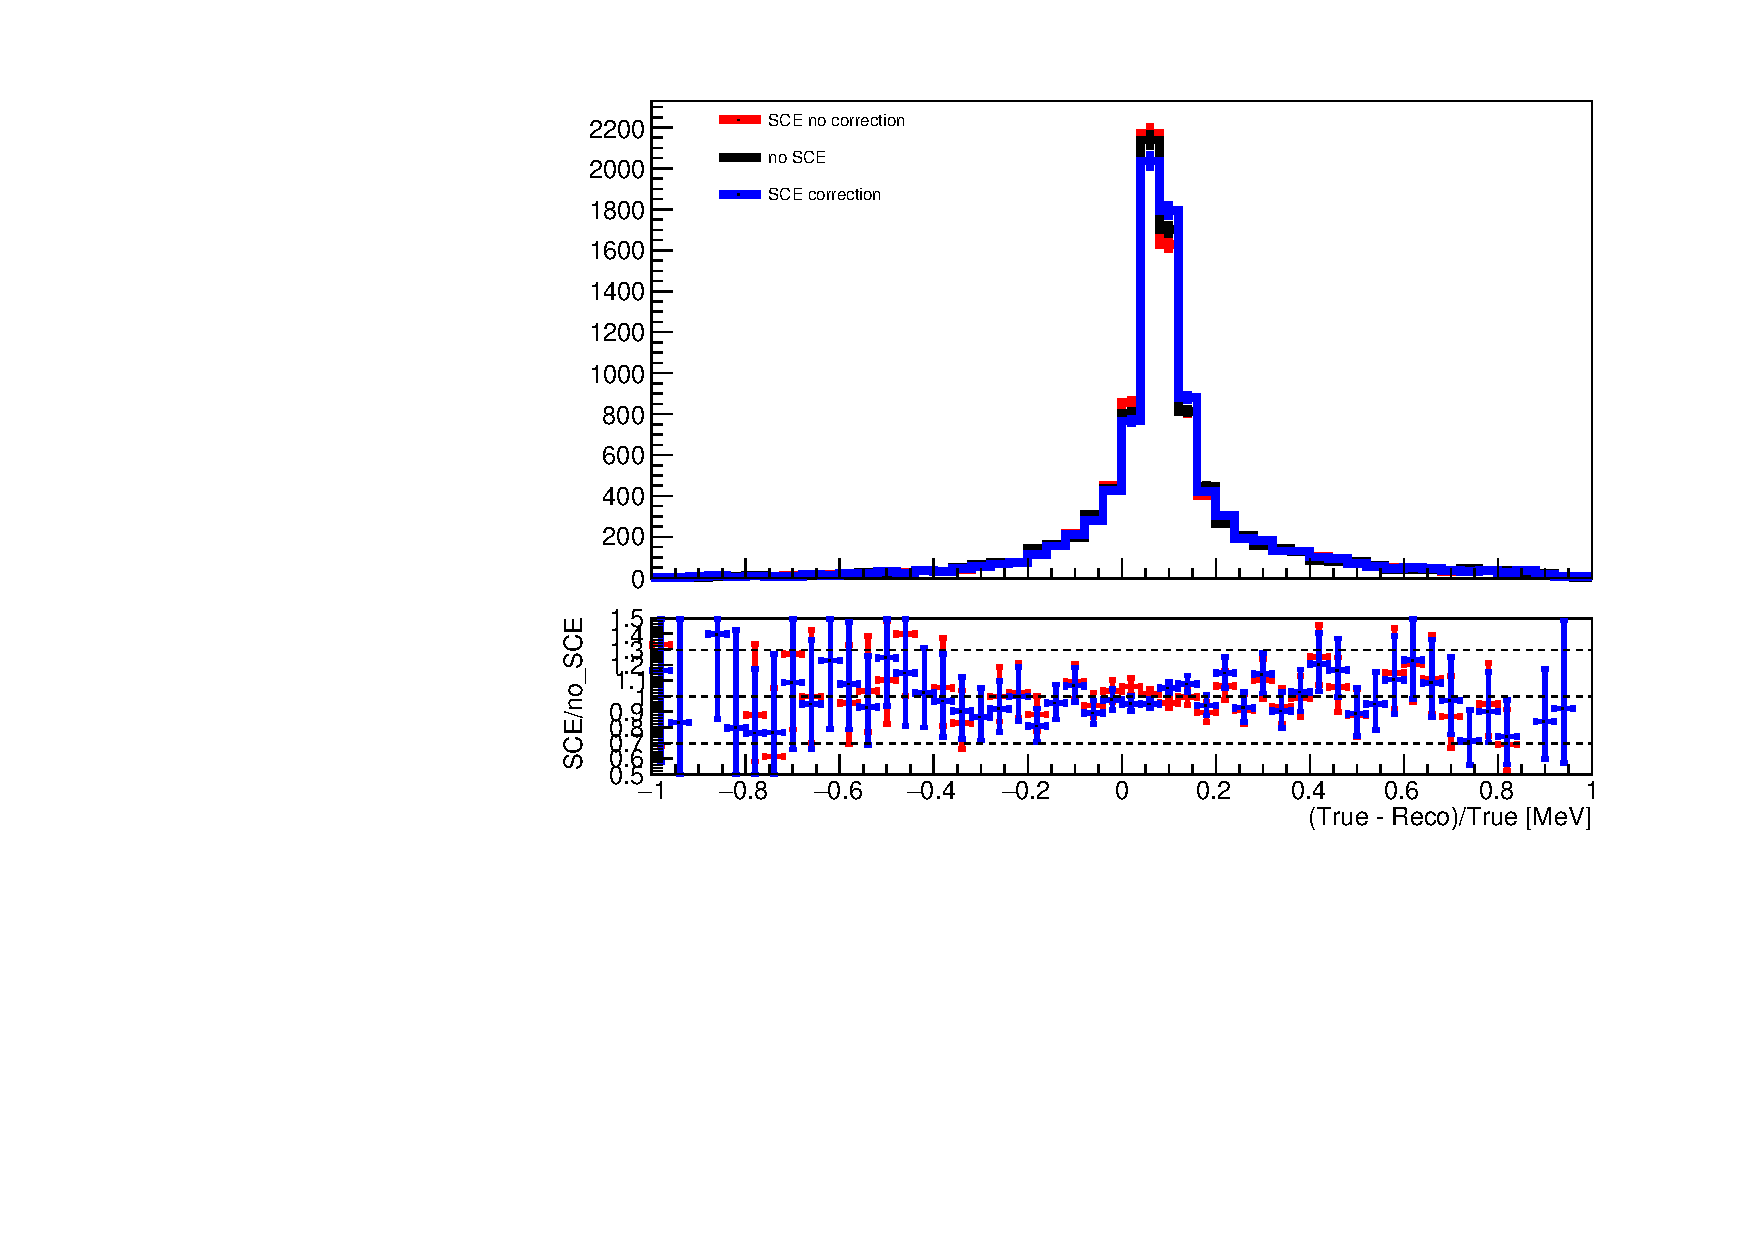
\includegraphics[width = \largefigwidth]{figures-chap4/ratio_plot_oldmethod_trueshoweringparticle.pdf}
    \caption{Caption}
    \label{fig:my_label}
\end{figure}



Shortcoming (don't know how much to put here? don't know if i want to emphasise how bad stuff is..): 
\begin{itemize}
    \item Things revolve around the nominal recomb of 0.64 - not really that realistic. 
    \item Correcting for SCE 'properly' is not straightforward either - using a fixed nominal dE/dx isn't ideal.
\end{itemize}

\end{comment}

\subsection{ESTAR Method}
The \textit{Shower ESTAR Energy tool} combines the ESTAR database provided by the \gls{nist} along with the Modified Box recombination model in an approach that was first used by the \Gls{argoneut} experiment \cite{ArgoNeuT_ESTAR_paper}. The ESTAR database provides the track length of electrons in various materials, including liquid argon, for energies ranging from 0.01 MeV to 1000 MeV \cite{ESTAR_Database}.

$\frac{dE}{dx}$ values may be calculated by dividing the energy by the track length for each entry in the ESTAR database. The deposited charge, \textit{Q}, can then found by using \EquationRef{eqn:ModBox} to find $\frac{dQ}{dx}$ and multiplying by the track length, \textit{dx}. This now allows the collected charge and energy to be related. If $\mathcal{E}$ in \EquationRef{eqn:ModBox} is taken to be a variable, the above process may be repeated whilst iterating over a set values of $\mathcal{E}$. This results in a 3D curve relating both the deposited charge and electric field to energy as is shown in \FigureRef{fig:ESTAR lookup curve}. The energy may then be interpolated from the collected charge and the appropriate electric field. As with the \textit{Shower Linear Energy tool}, a direct correction for recombination isn't needed as it is again accounted for in the lookup curve. 

\begin{figure}[h]
    \centering
    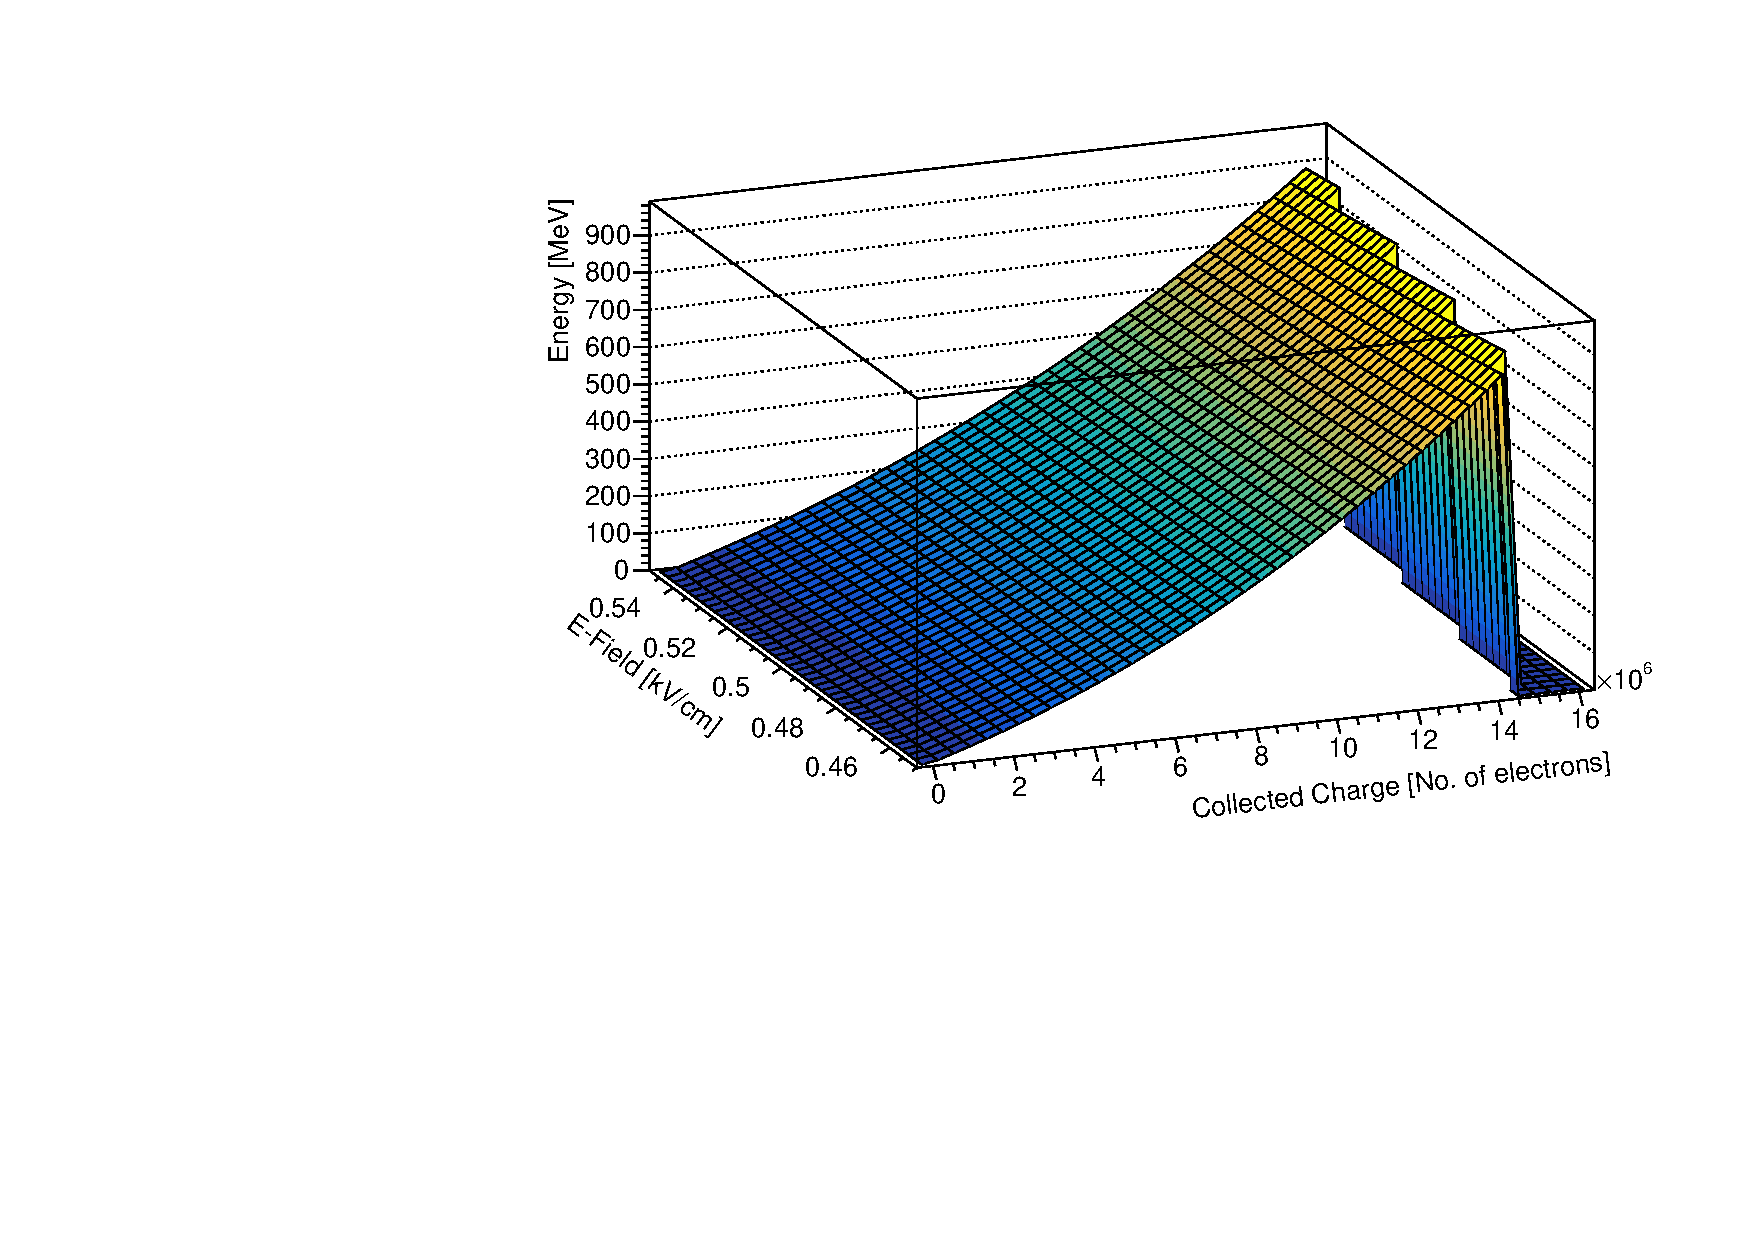
\includegraphics[width = 0.8\textwidth]{figures-chap4/ESTAR_lookup_curve.pdf}
    \caption{ESTAR Lookup Curve}
    \label{fig:ESTAR lookup curve}
\end{figure}

\section{Shower Energy Reconstruction Performance}

In order to assess the performance of the different reconstruction methods, a comparison with \textit{truth} information is performed. Depending on the approach, a few other inefficiencies should be considered, namely that the hit reconstruction and Pandora pattern recognition aren't perfect. This results in hits missing due to not being reconstructed plus the addition of the clusters that Pandora produces being incomplete. Therefore, there are typically fewer hits than there would be if the the shower in question were to be perfectly reconstructed. Reconstructing the energy of the showering particle, is desirable for a number of analyses, however, due to these issues, it is not realistic to expect agreement to within a few percent. Improving the hit reconstruction or the pattern recognition within Pandora would clearly help, but it's likely that a non-negligible bias would remain. Work on Pandora and the hit reconstruction is, however, beyond the scope of this section and addressing any remaining bias between true and reco is beyond reconstruction work as a whole. 

To purely gauge the performance of a given reconstruction method, it is probably best to compare the truth and reconstructed energy of a shower by only considering the available hits. This way, the reconstruction method is only validated from the available information and is decoupled from any other inefficiencies. However, additional care must be taken when using the true energy of the hits. What is considered a hit is user defined in that the width that defines a hit is a parameter that may be changed. Therefore, the true energy associated with a hit is dependant on the chosen width. Within \gls{larsoft}, the default width of a hit is $1\sigma$ which is chosen to try and find a balance between covering a sufficient amount of charge whilst still being able to resolve multiple hits which are closely spaced. Unless otherwise stated, the definition of a hit will be left at the default width of $1\sigma$. 

Generally the validation is performed on a shower-hit level. This means that for a given shower, the energy of each hit is reconstructed and then the summed together to obtain the energy of the shower. The exception to this is in the case of the \textit{Linear Energy tool}. During its development, it was customary to sum up the charge of all the hits and then convert to energy. This is why the calibration curve in \FigureRef{fig:linear lookup curve} has energies on the order of a shower level and not a hit level (individual hit energies are usually $\lesssim 5$ MeV).

\subsection{General Validation of a BNB Sample}

In order to validate the reconstruction methods, an $e^- + \pi^+$ vertex sample with \gls{bnb}-like properties was produced where the electron is the showering particle. \textcolor{red}{WHY DO WE USE VERTEX SAMPLE?? HELPS PANDORA, BUT WHY..}

The true vs reconstructed energy is shown in \FigureRef{fig:reco_vs_true_hit_level} for all three methods where the true energy has been calculated from the shower hits. The results from the \textit{Shower Linear Energy tool} and the \textit{Shower ESTAR Energy tool} are similar and show good agreement between true and reconstructed energies across the whole energy range whereas the \textit{Shower Num Electrons Energy tool} tends to overestimate the hit energies. \FigureRef{fig:reco_vs_true_showeringE} is similar, but instead the true energy is the energy of the showering electron. This gives a measure of the bias each method can expect due to the inefficiencies mentioned above. Both the \textit{Shower Linear Energy tool} and the \textit{Shower ESTAR Energy tool} underestimate the true energy of the showering electron as is expected. The \textit{Shower Num Electrons Energy tool} shows better agreement due to systematically applying a higher energy to individual hits which compensates for other inefficiencies. 

\begin{figure}[h!]
    \centering
    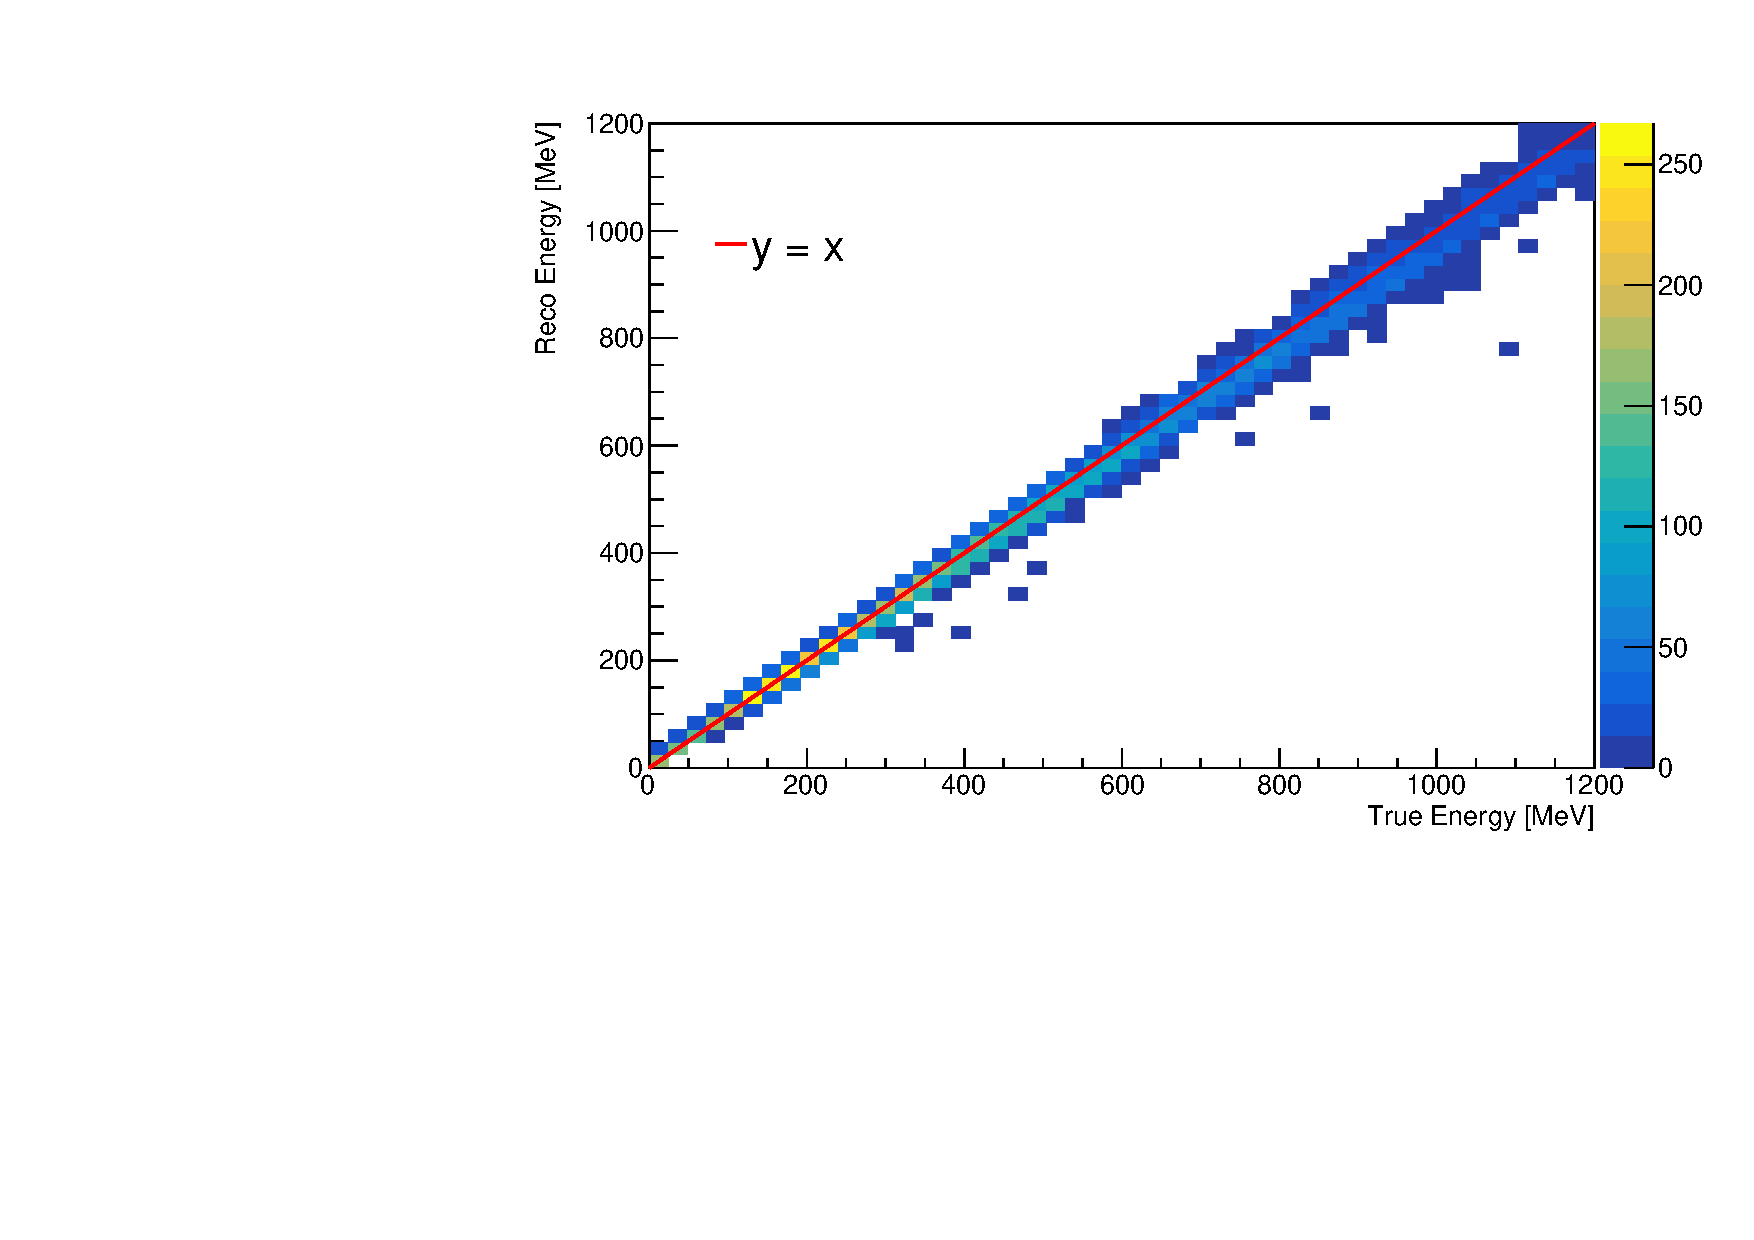
\includegraphics[width = 0.49\textwidth]{figures-chap4/true_vs_reco_linear.pdf}
    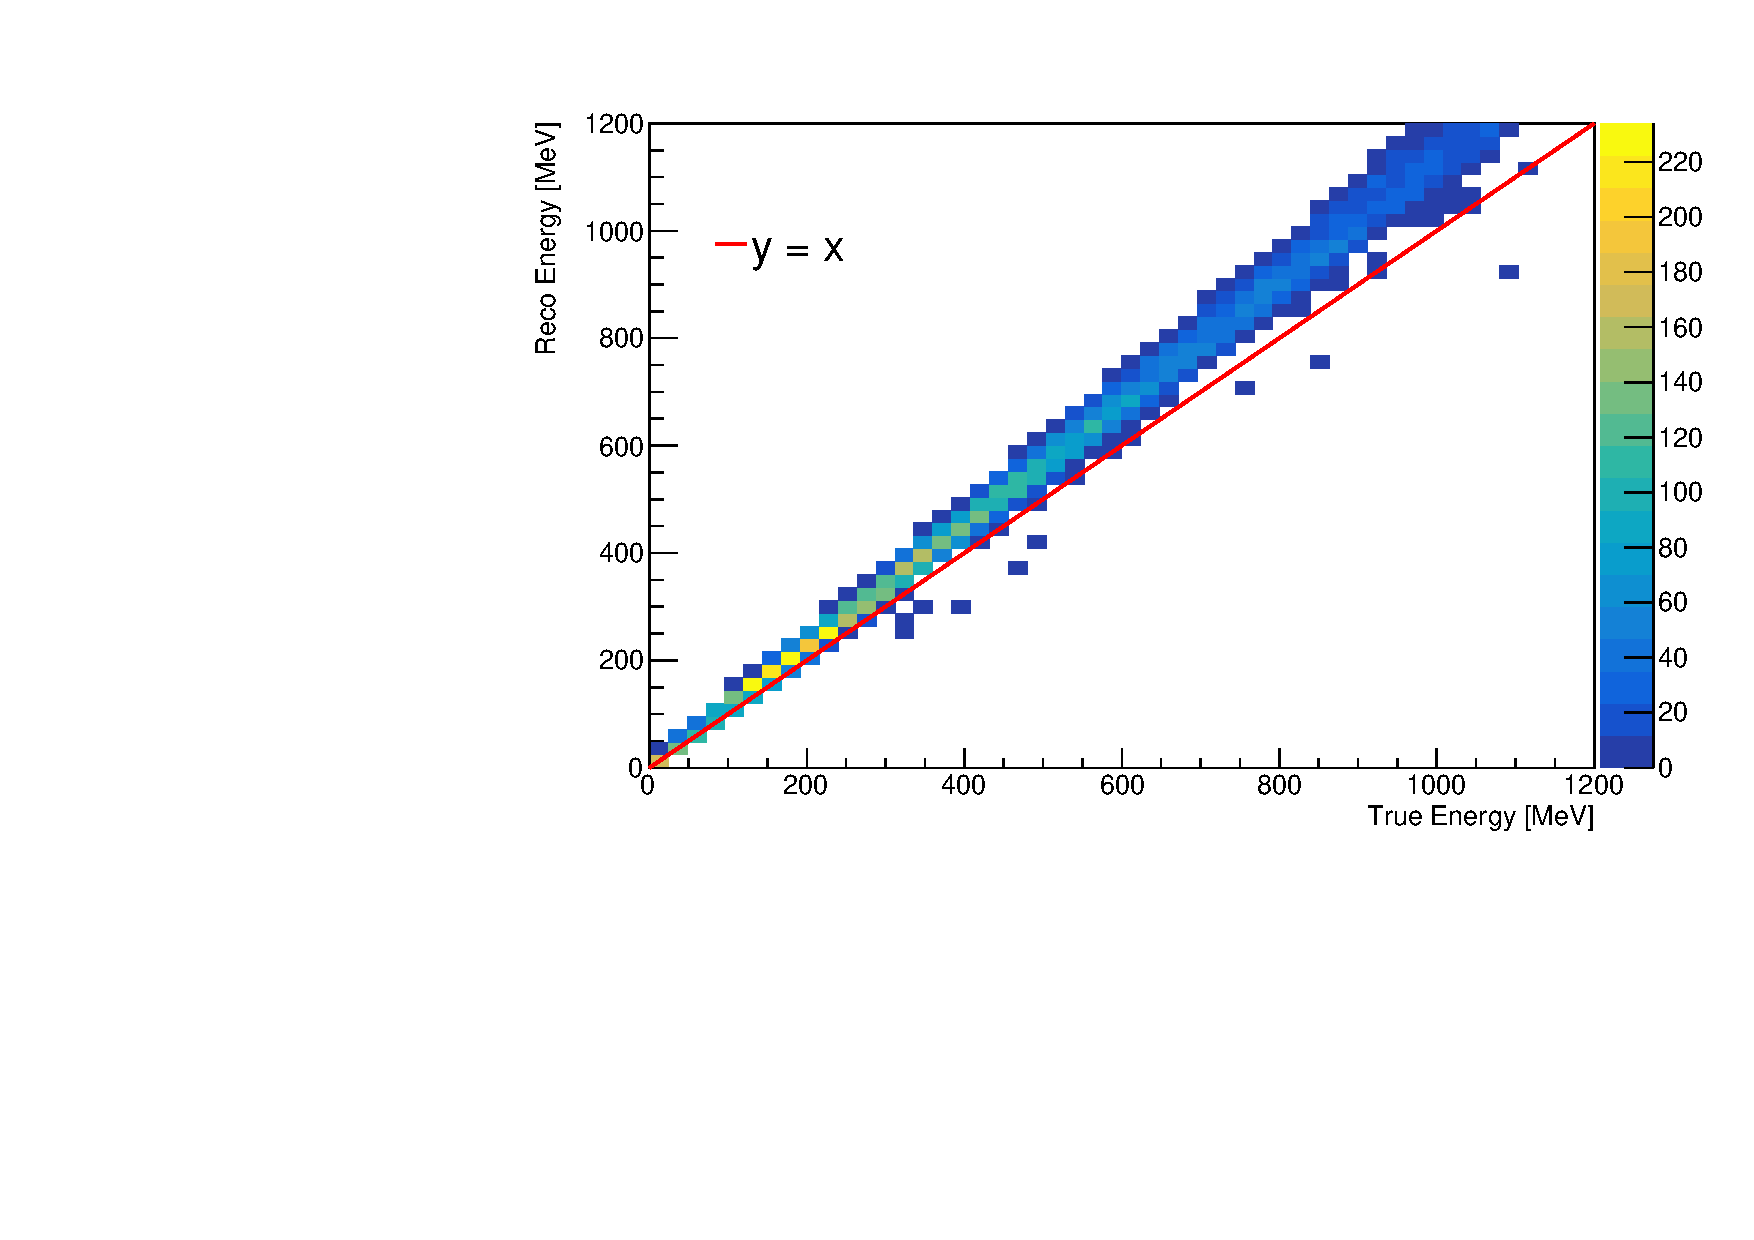
\includegraphics[width = 0.49\textwidth]{figures-chap4/true_vs_reco_oldmethod.pdf}
    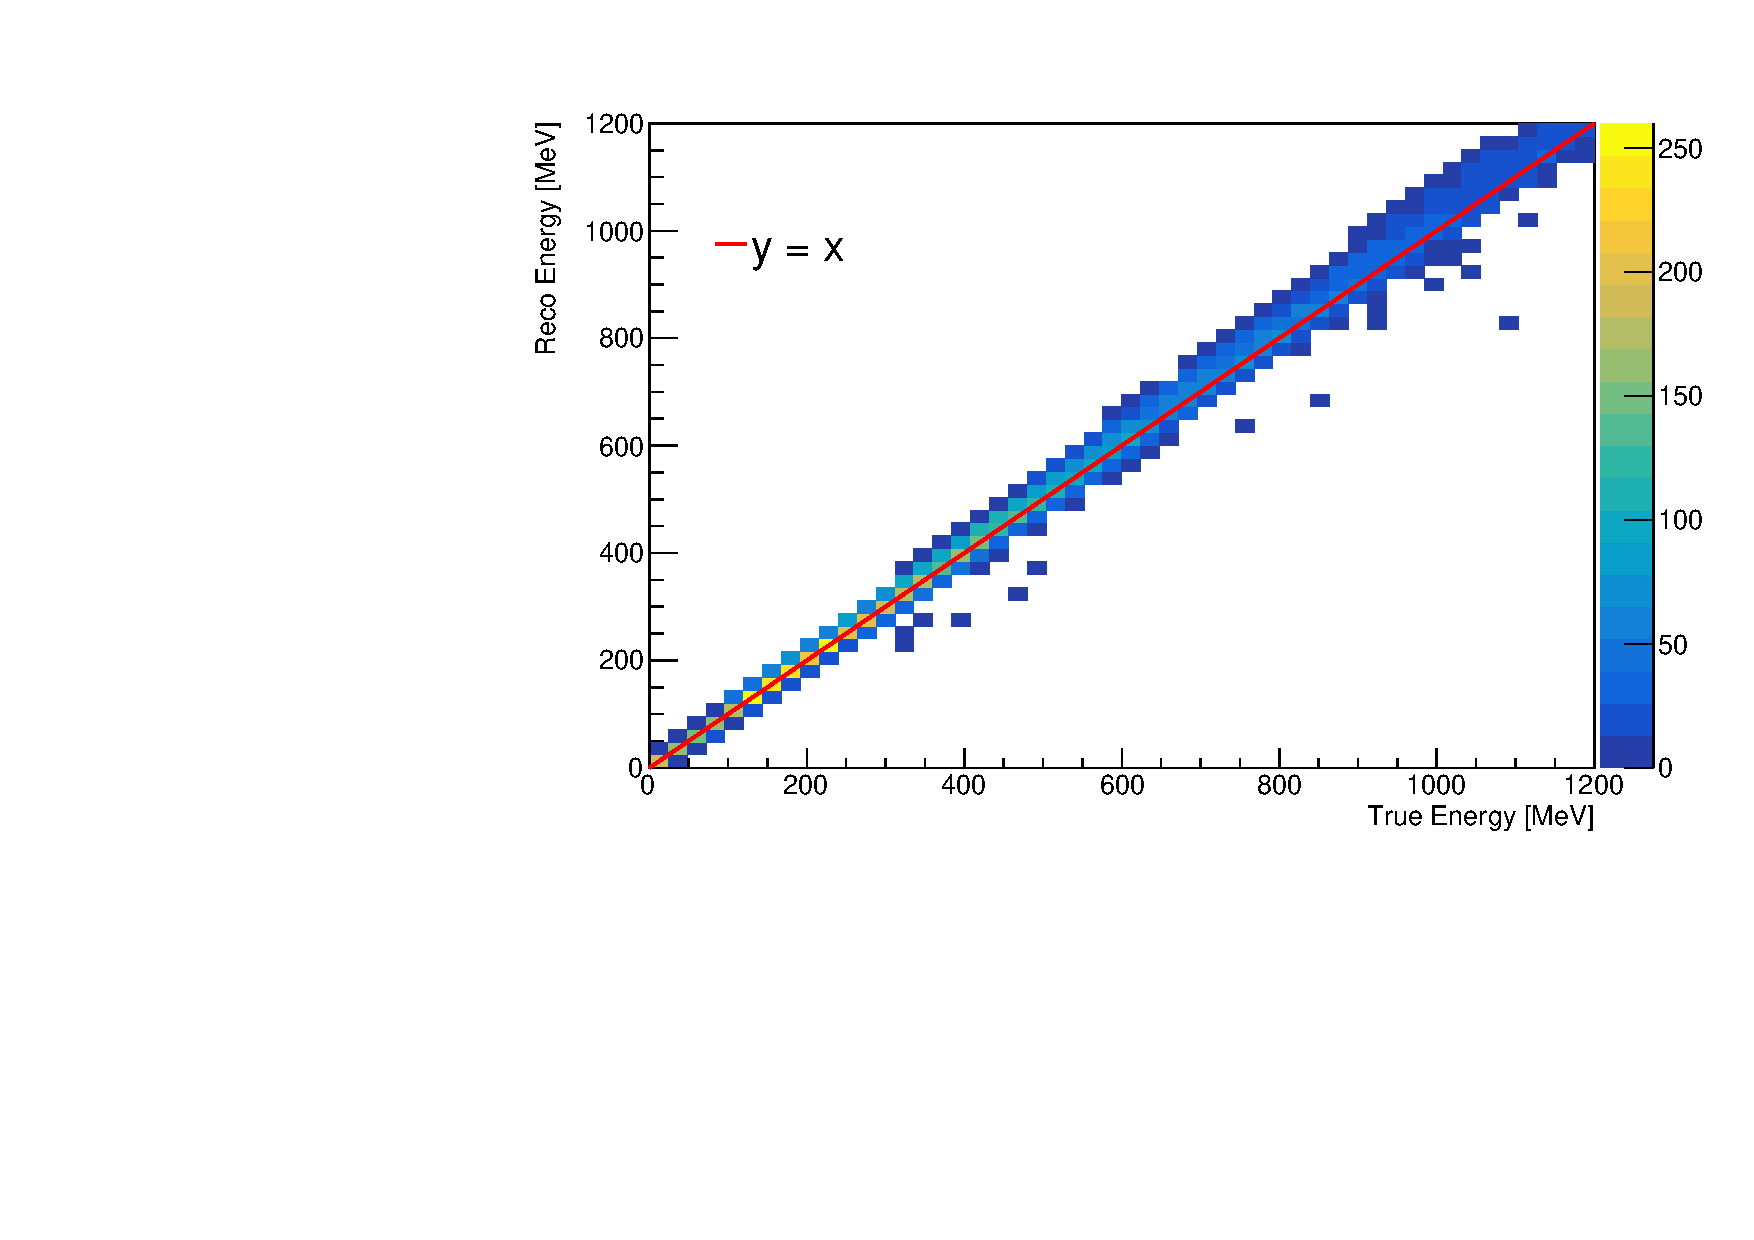
\includegraphics[width = 0.49\textwidth]{figures-chap4/true_vs_reco_ESTAR.pdf}
    \captionsetup{width=0.45\textwidth}
    \parbox[b]{0.49\textwidth}%
  {
    \caption[Reconstructed vs true shower energy. The true energy has been evaluated from the hits of each shower.]
    {Reconstructed vs true shower energy. The true energy has been evaluated from the hits of each shower. Top Left: \textit{Shower Linear Energy tool}, Top Right: \textit{Shower Num Electrons Energy tool} and Bottom Left: \textit{Shower ESTAR Energy tool}. \\\\}
    \label{fig:reco_vs_true_hit_level}}
\end{figure}


\begin{figure}[h!]
    \centering
    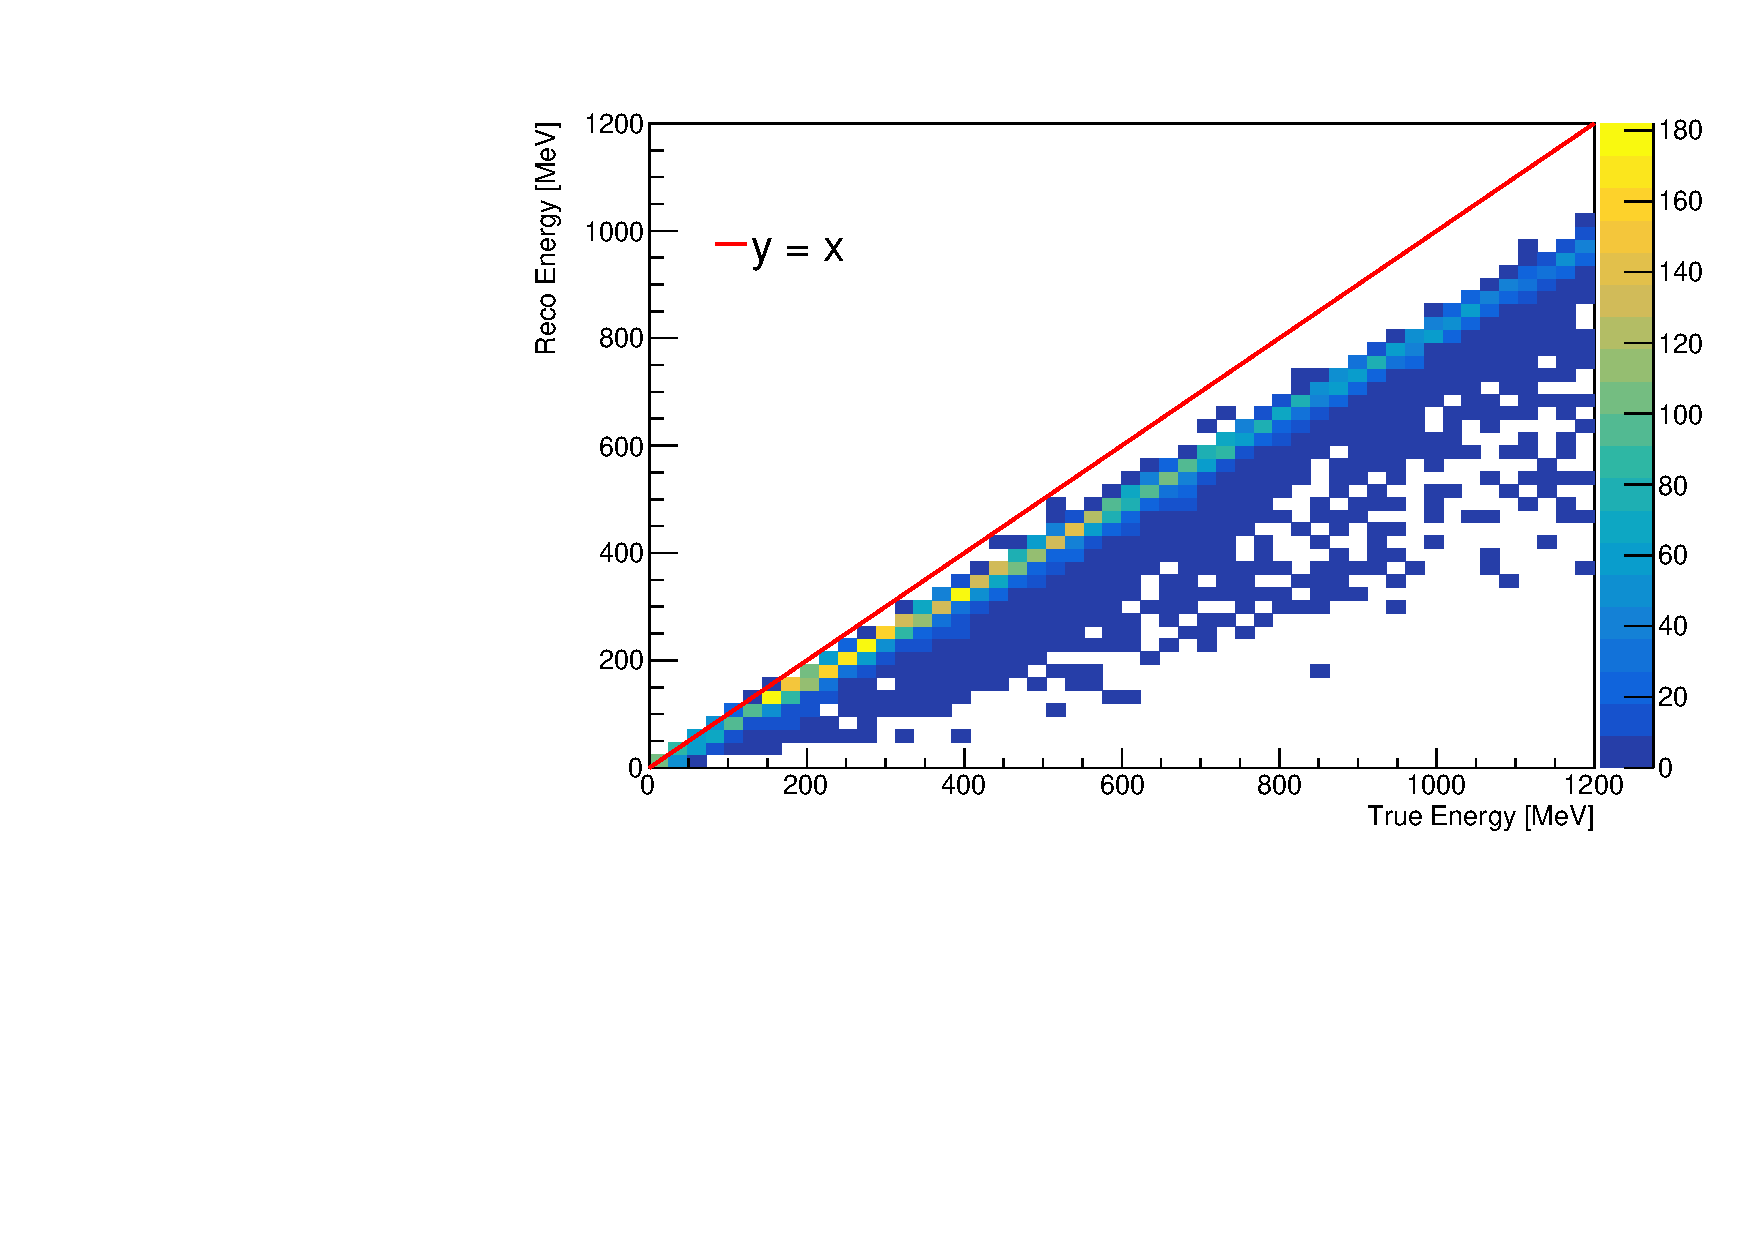
\includegraphics[width = 0.49\textwidth]{figures-chap4/true_vs_reco_showeringE_linear.pdf}
    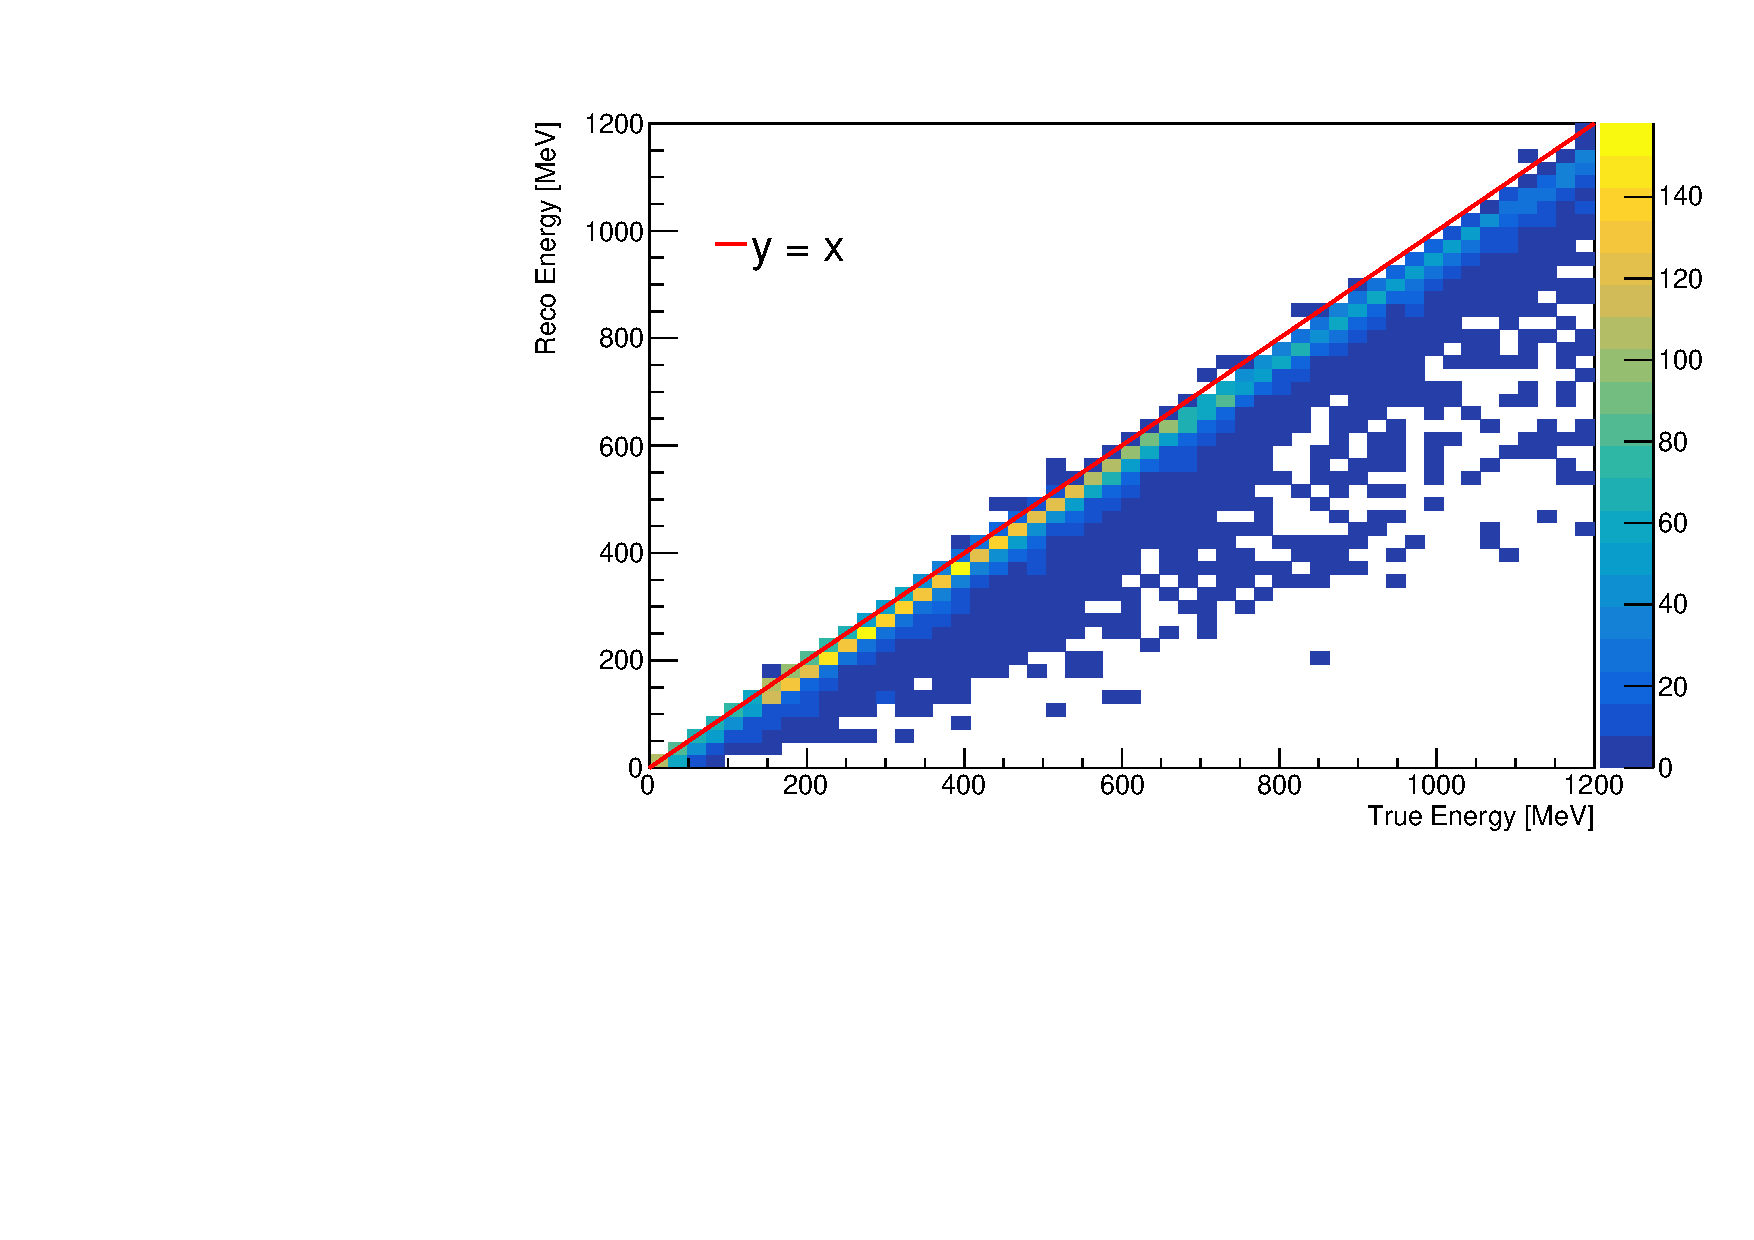
\includegraphics[width = 0.49\textwidth]{figures-chap4/true_vs_reco_showeringE_oldmethod.pdf}
    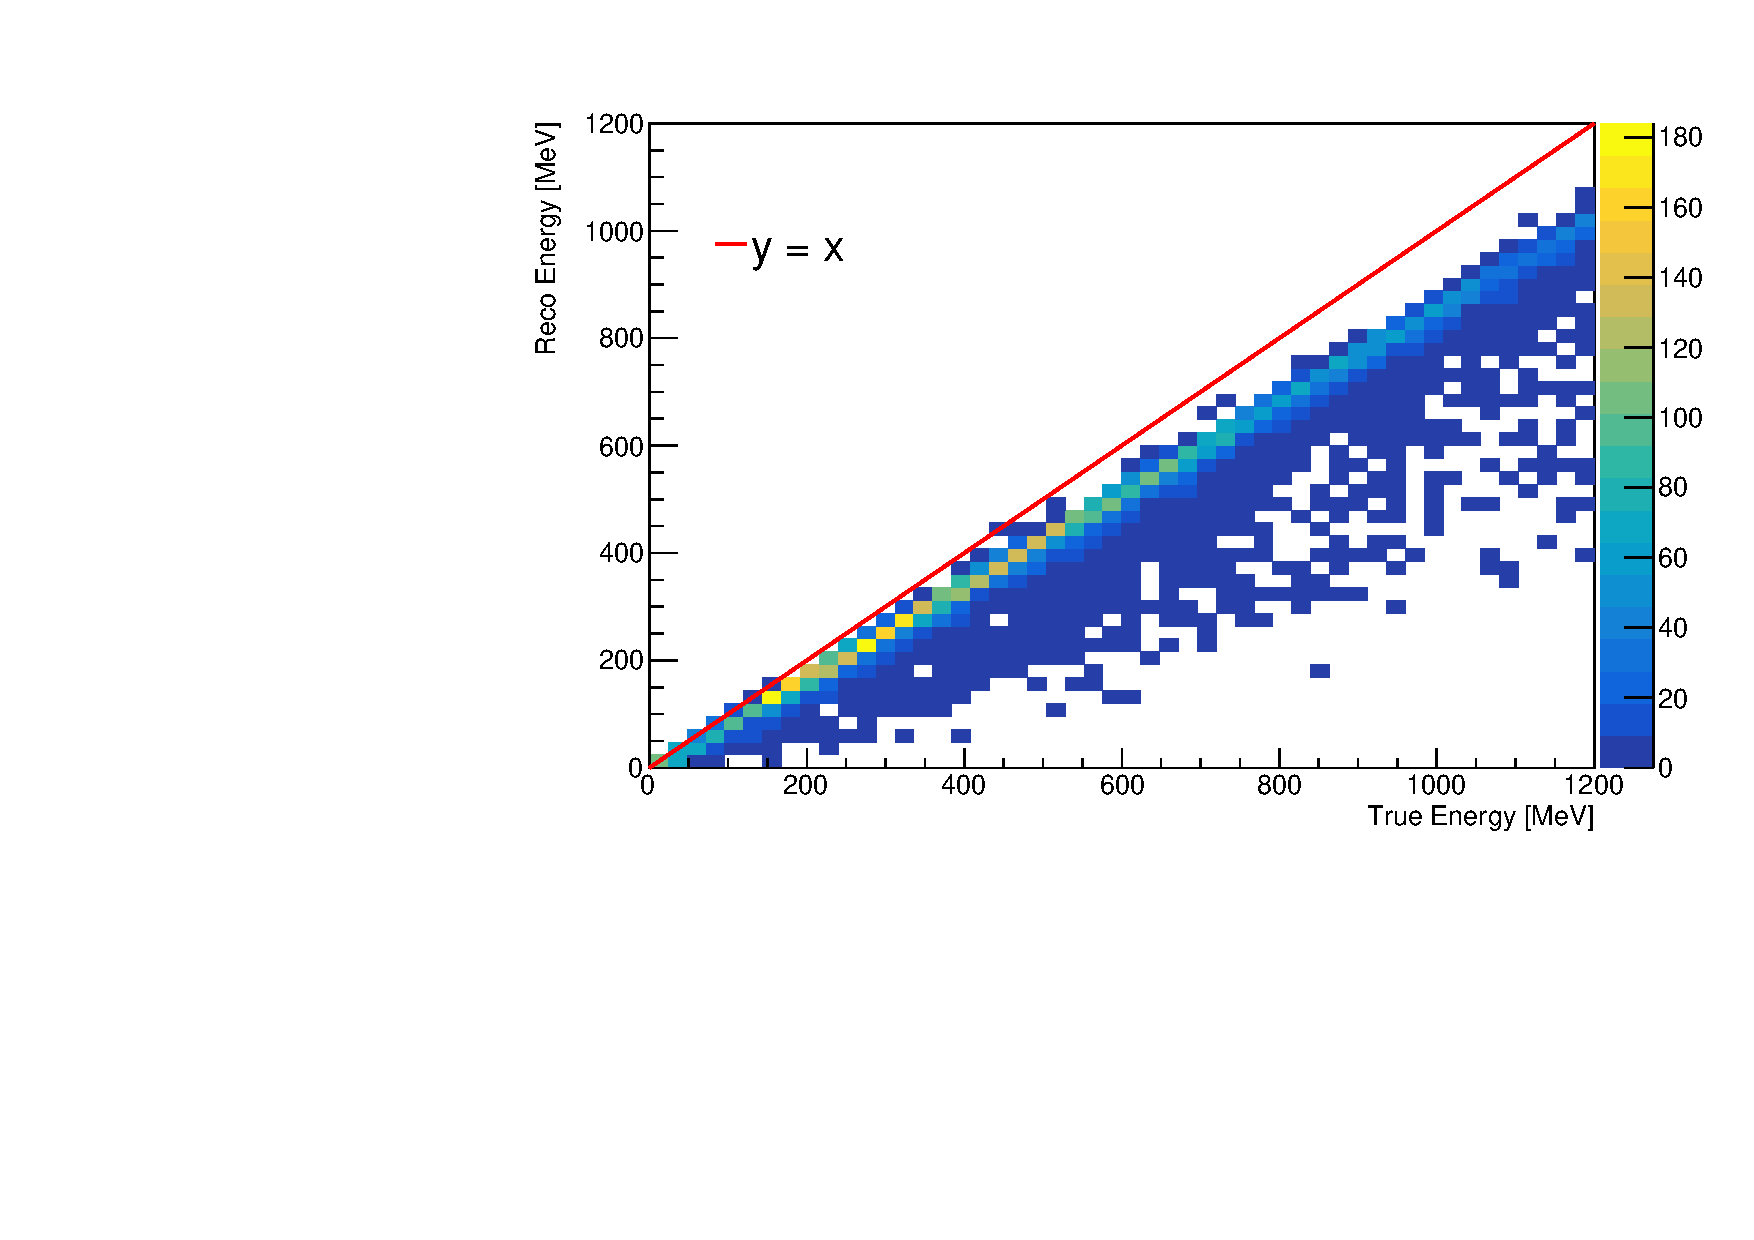
\includegraphics[width = 0.49\textwidth]{figures-chap4/true_vs_reco_showeringE_ESTAR.pdf}
    \captionsetup{width=0.45\textwidth}
    \parbox[b]{0.49\textwidth}%
  {
    \caption[Reconstructed vs true shower energy. The true energy is the energy of the showering electron.]
    {Reconstructed vs true shower energy. The true energy is the energy of the showering electron. Top Left: \textit{Shower Linear Energy tool}, Top Right: \textit{Shower Num Electrons Energy tool} and Bottom Left: \textit{Shower ESTAR Energy tool}. \\\\}
    \label{fig:reco_vs_true_showeringE}}
\end{figure}

A comparison of the fractional energy resolution, which is defined as $\frac{Reco - True}{True}$, is shown in \FigureRef{fig:fractional_energy_resolution_hit_level}.

\begin{figure}[h!]
    \centering
    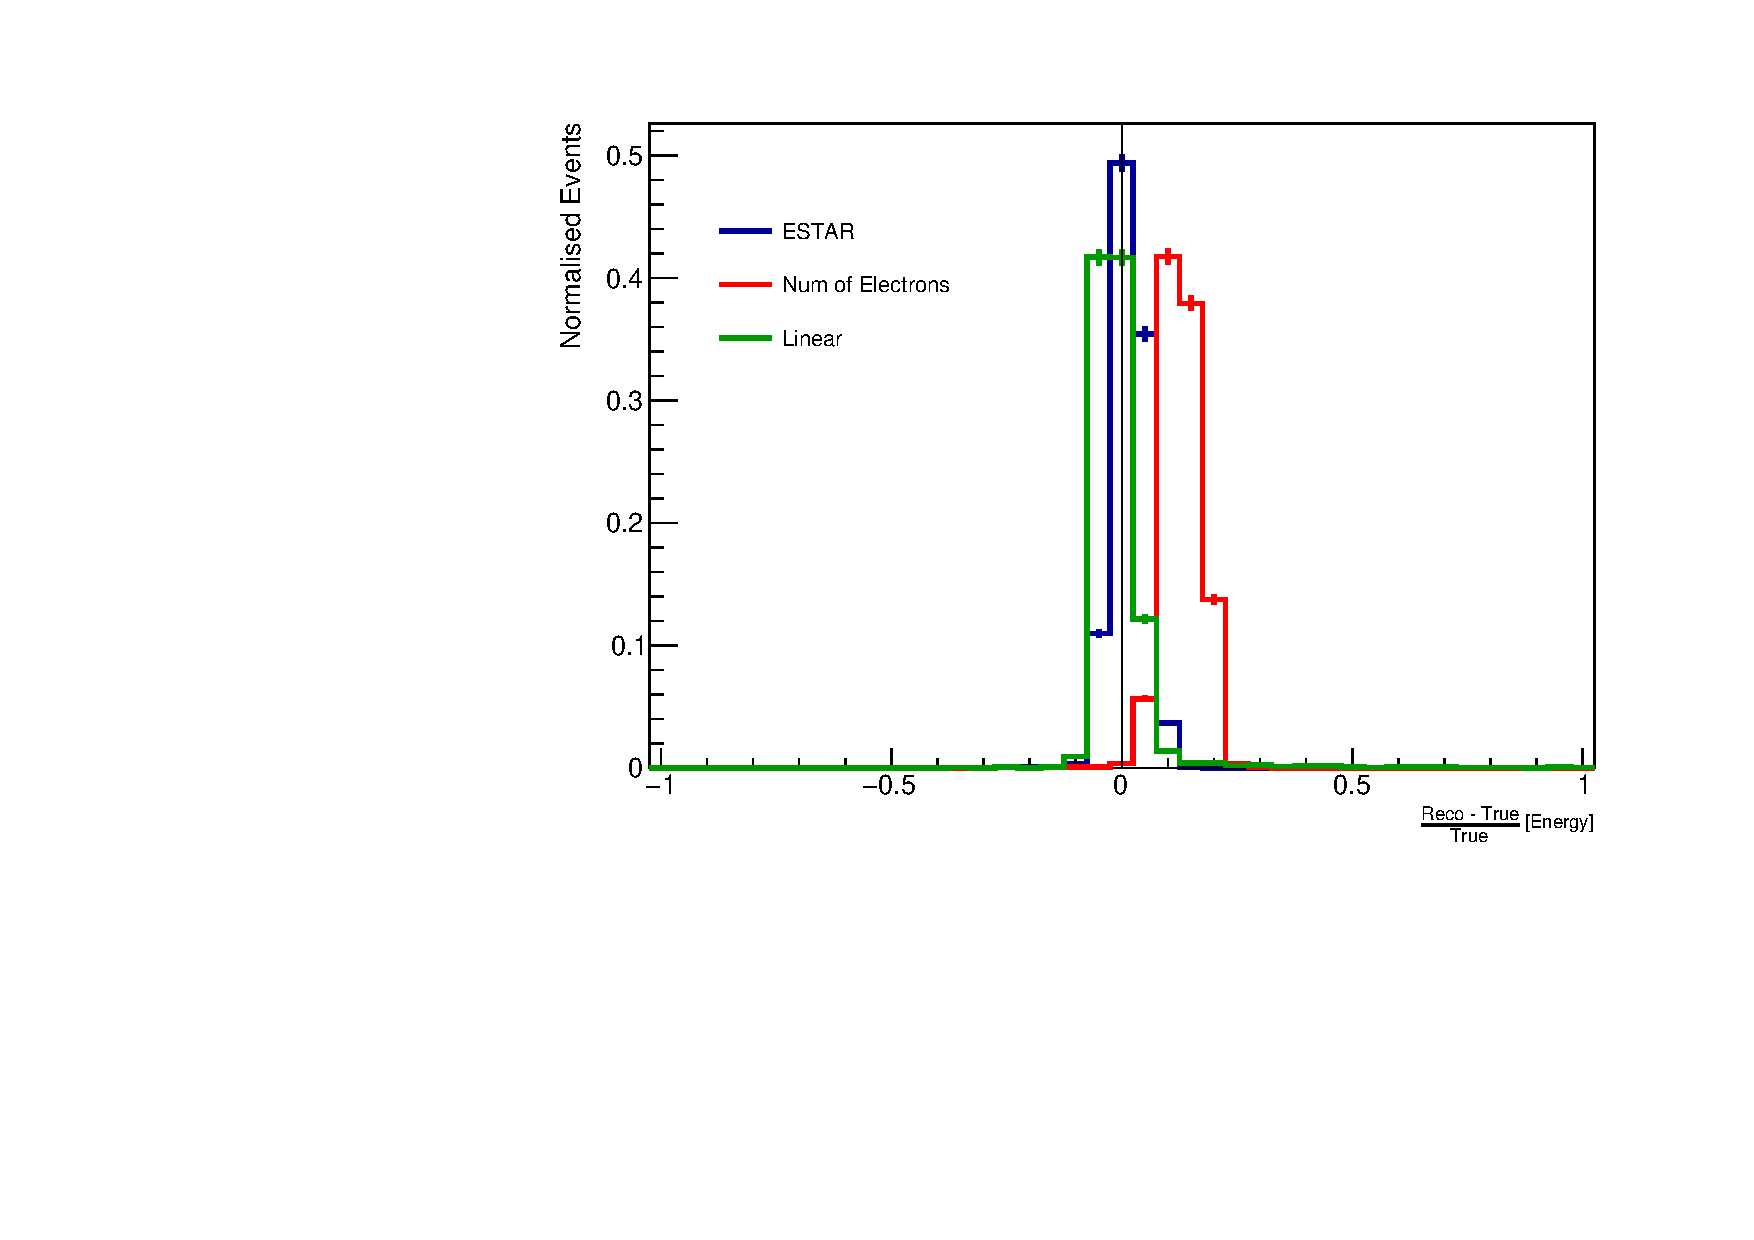
\includegraphics[width = \largefigwidth]{figures-chap4/bias_cheat_plane_2_all.pdf}
    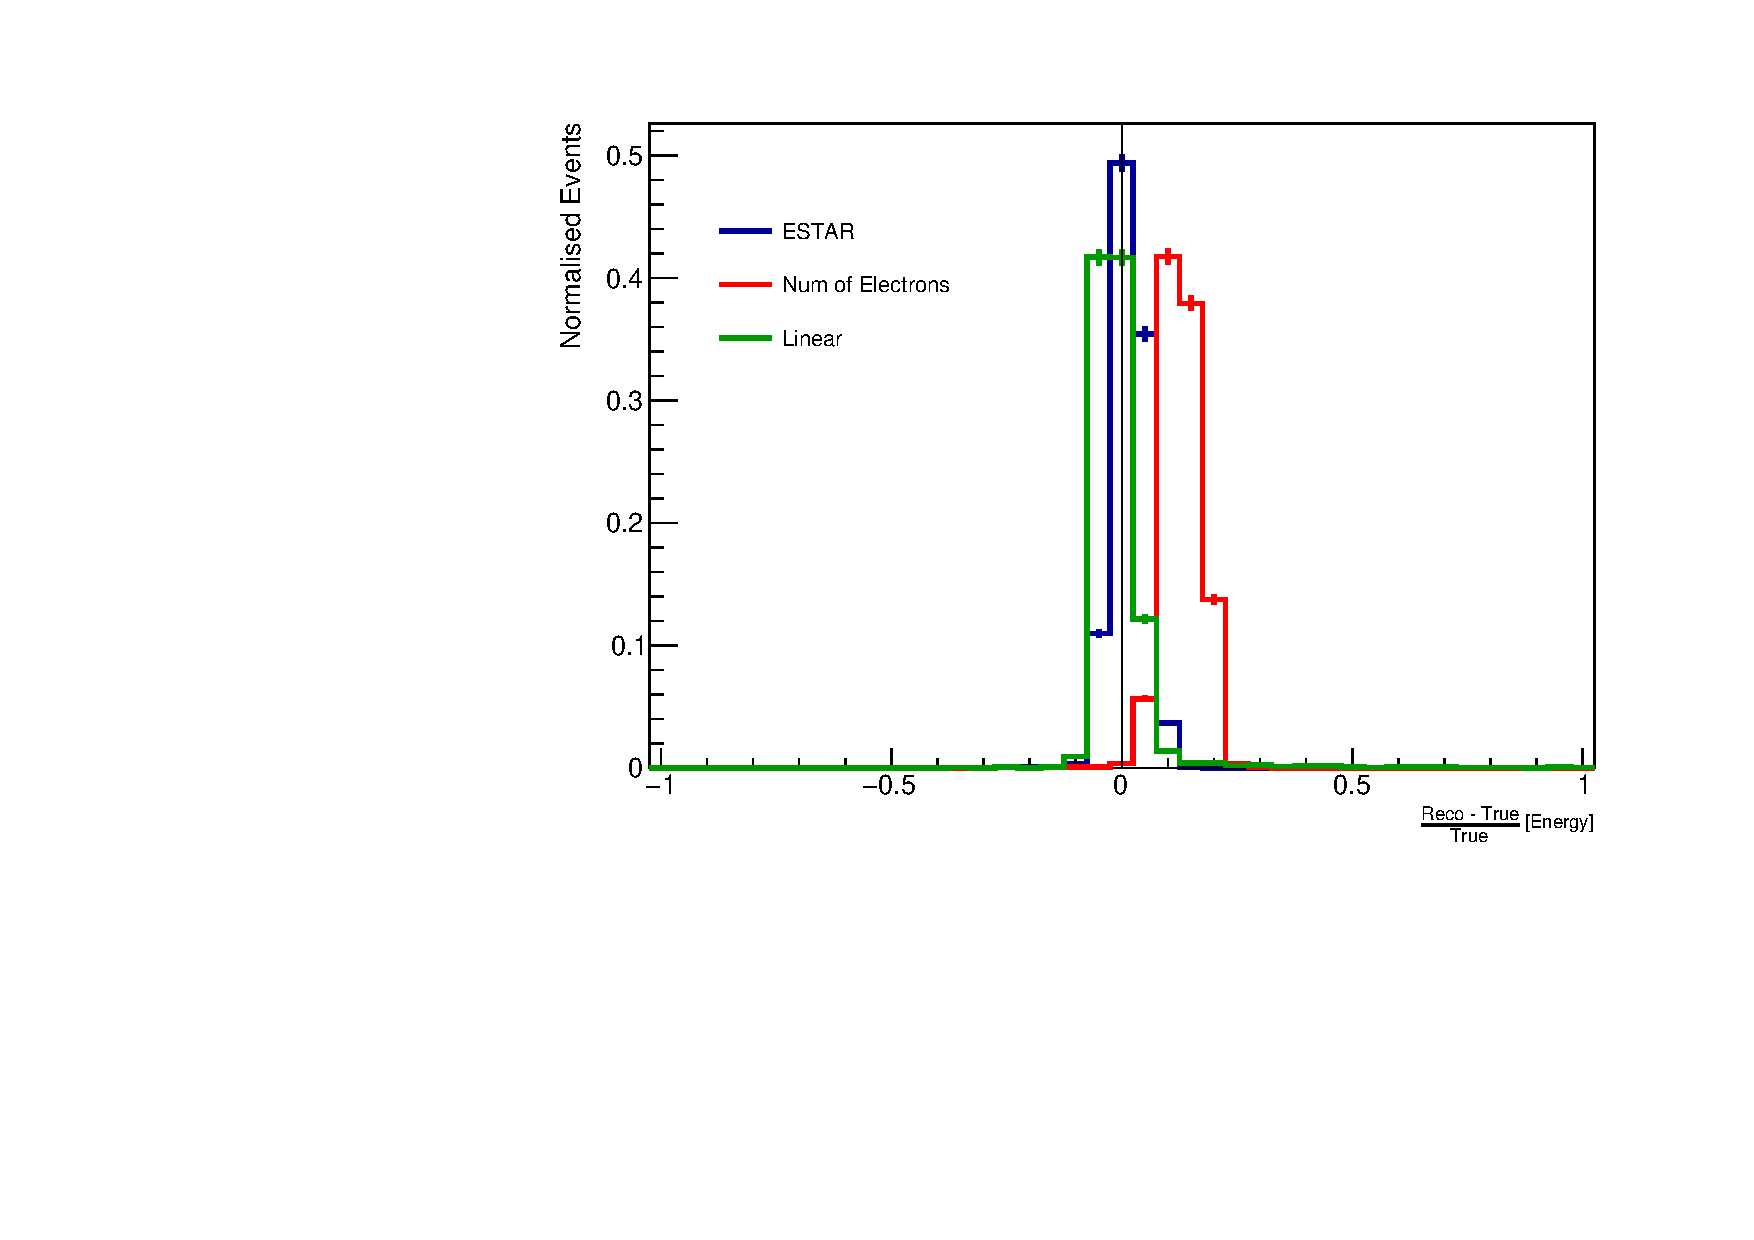
\includegraphics[width = \largefigwidth]{figures-chap4/bias_cheat_plane_2_all.pdf}
    \caption[Comparison of the reconstructed fractional shower energy resolution.]{Comparison of the reconstructed fractional shower energy resolution for the \textit{Shower Linear Energy tool}, the \textit{Shower Num Electrons Energy tool} and the \textit{Shower ESTAR Energy tool}. Left: Using the true energy of the hits. Right: Using the true energy of the showering particle.}
    \label{fig:fractional_energy_resolution_hit_level}
\end{figure}

\clearpage
\subsection{Performance as a Function of Angle}

From a \gls{bnb} neutrino sample, most of the showers are expected to be predominantly forward going. A fraction of showers will however be directed at large angles to the beamline. As was mentioned in \SectionRef{sec:Event Production and Reconstruction in LArSoft}, showers directed towards the wire planes tend to produce waveforms which are not well represented by Gaussians. Since the GausHitFinder has trouble applying a suitable fit to these cases, a degradation in the reconstruction performance is expected as a function of angle.

In order to verify this, an  $e^- + \pi^+$ sample was produced with the electron being directed in all $\theta_{xz}$ angles. Otherwise, this sample is also \gls{bnb}-like. $\theta_{xz}$ is the angle between the beamline and the positive x-direction and is defined in terms of \glspl{sbnd} coordinate system which is shown in \FigureRef{fig:sbnd_coordinate_system}. The reconstruction performance is shown in \FigureRef{fig:reconstruction_as_a_function_of_angle} using the ESTAR method for both definitions of true energy. As is expected, a degradation in the reconstruction performance is observed in both cases as $\theta_{xz}$ tends away from 0. It should be noted that the degradation's are in opposite directions which may be explained by the fact that at large angles, the reconstruction method tends to overestimate the energy of the available hits, but the hit reconstruction and/or clustering also suffer, so the overall fraction of hits representing the shower is reduced. Both the \textit{Shower Linear Energy tool} and \textit{Shower Num Electrons Energy tool} have a constant recombination correction and therefore the conversion from charge to energy is linear. The \textit{Shower ESTAR Energy tool} isn't perfectly linear but it is close, especially in the region up to $\mathcal{O}(10 \text{ MeV})$. Therefore, there is essentially no angular dependence so results akin to \FigureRef{fig:reconstruction_as_a_function_of_angle} for the \textit{Shower Linear Energy tool} and the \textit{Shower Num of Electrons Energy tool} would look almost identical only with the y-axis scaled appropriately. 
\begin{figure}[h!]
    \centering
    
    \begin{tikzpicture}[x=1cm, y=1cm, z=-0.6cm]
        \draw (0,0) node (O) {};
        % Axes
        \draw [->] (0,0,0) -- (-4,0,0) node (x) [left, at end] {$x$}; %[above] {$x$};
        \draw [->] (0,0,0) -- (0,4,0) node (y) [above] {$y$};
        \draw [->] (0,0,0) -- (0,0,-4) node [right, xshift=-0.25em, yshift=0.5em] (z) {$z$};
    
        \pic [draw=red, ->, "\textcolor{red}{$\theta_{xz}$}", angle radius=1.3cm, angle  eccentricity=1.3] {angle = z--O--x};
        \pic [draw=teal, ->, "\textcolor{teal}{$\theta_{yz}$}", angle radius=0.7cm, angle eccentricity=1.45] {angle = z--O--y};

    \end{tikzpicture}

    \caption[\glspl{sbnd} coordinate system]{\glspl{sbnd} coordinate system. The origin is located at the centre of the upstream face of the detector which is defined to be at (0, 200, 0) cm with the \textit{z} direction being along the beamline.}
    \label{fig:sbnd_coordinate_system}
\end{figure}


\begin{figure}
    \centering
    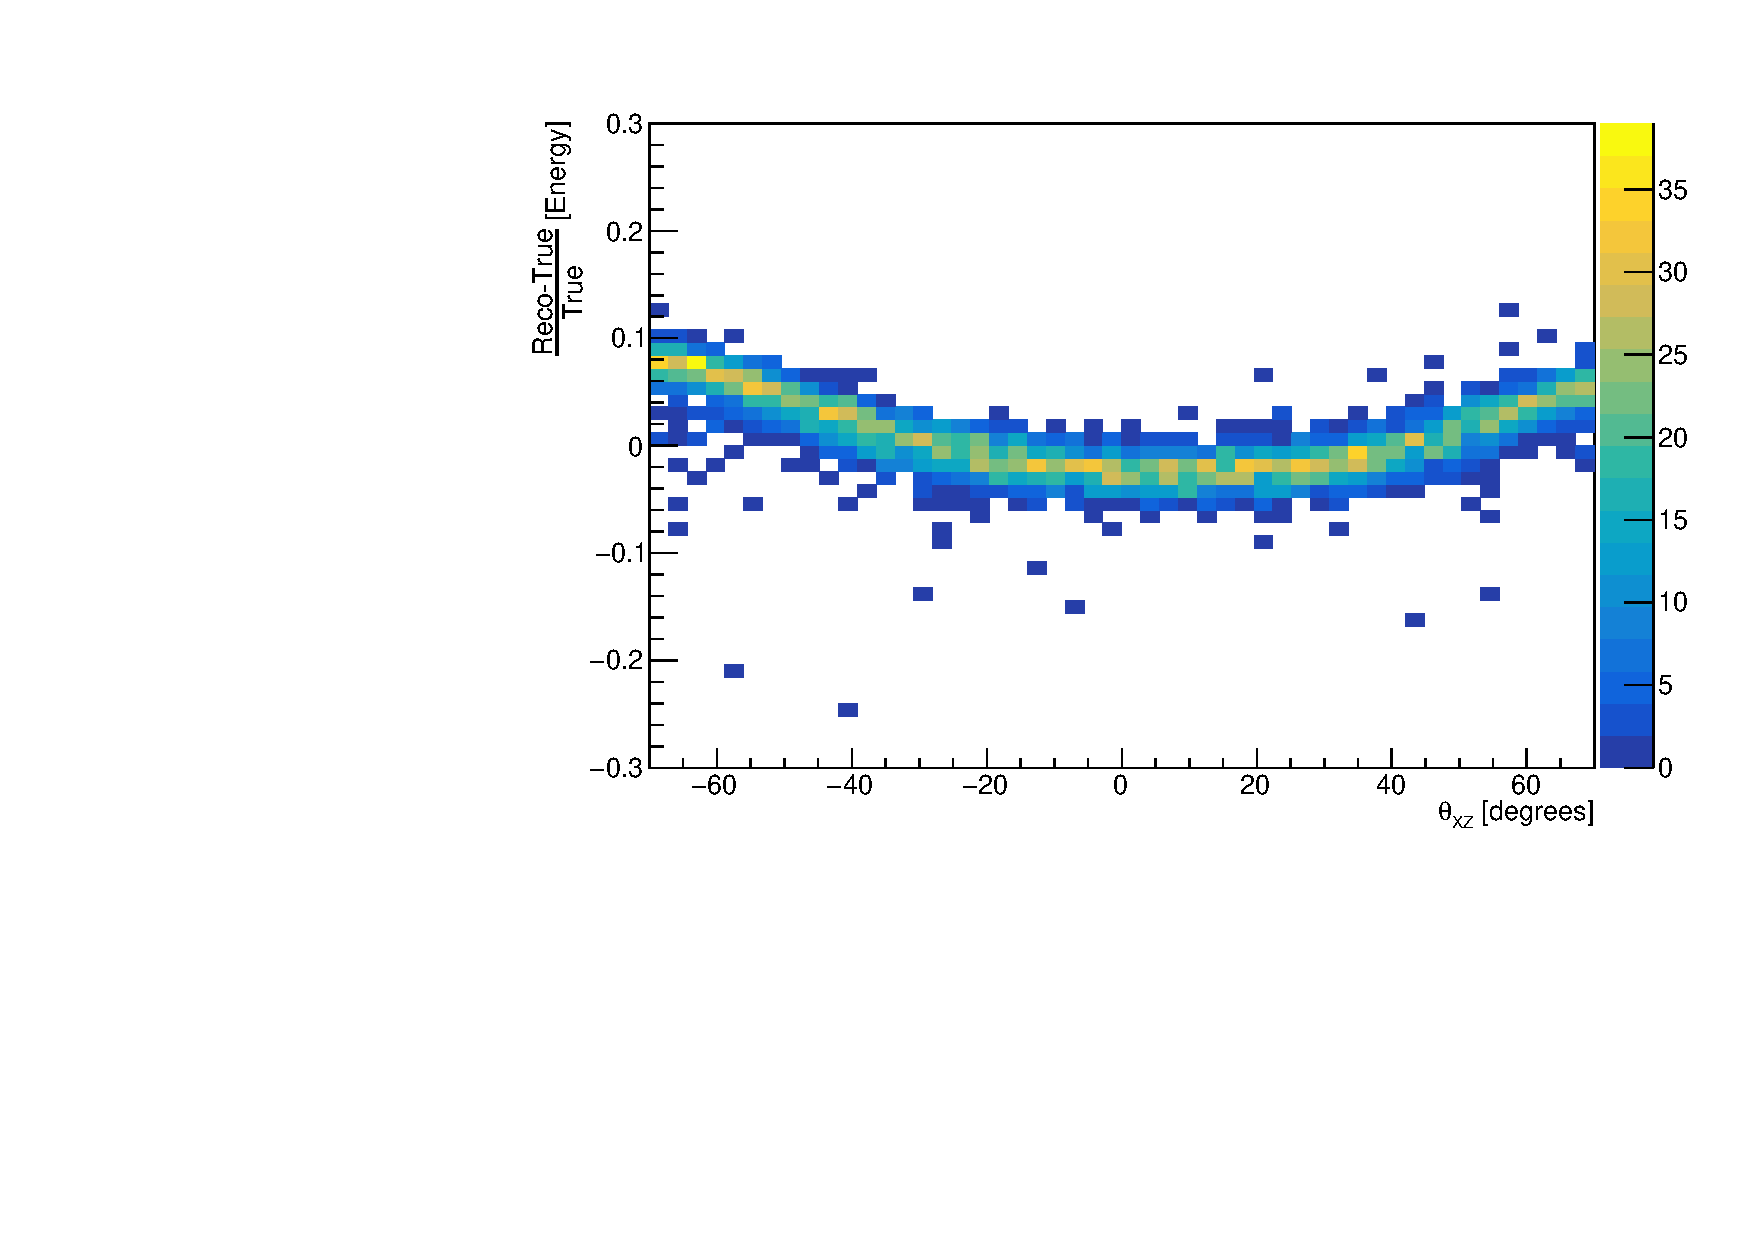
\includegraphics[width = 0.49\textwidth]{figures-chap4/frac_res_vs_thetaXZ_cheating_electron_vertex_plane2_cut.pdf}
    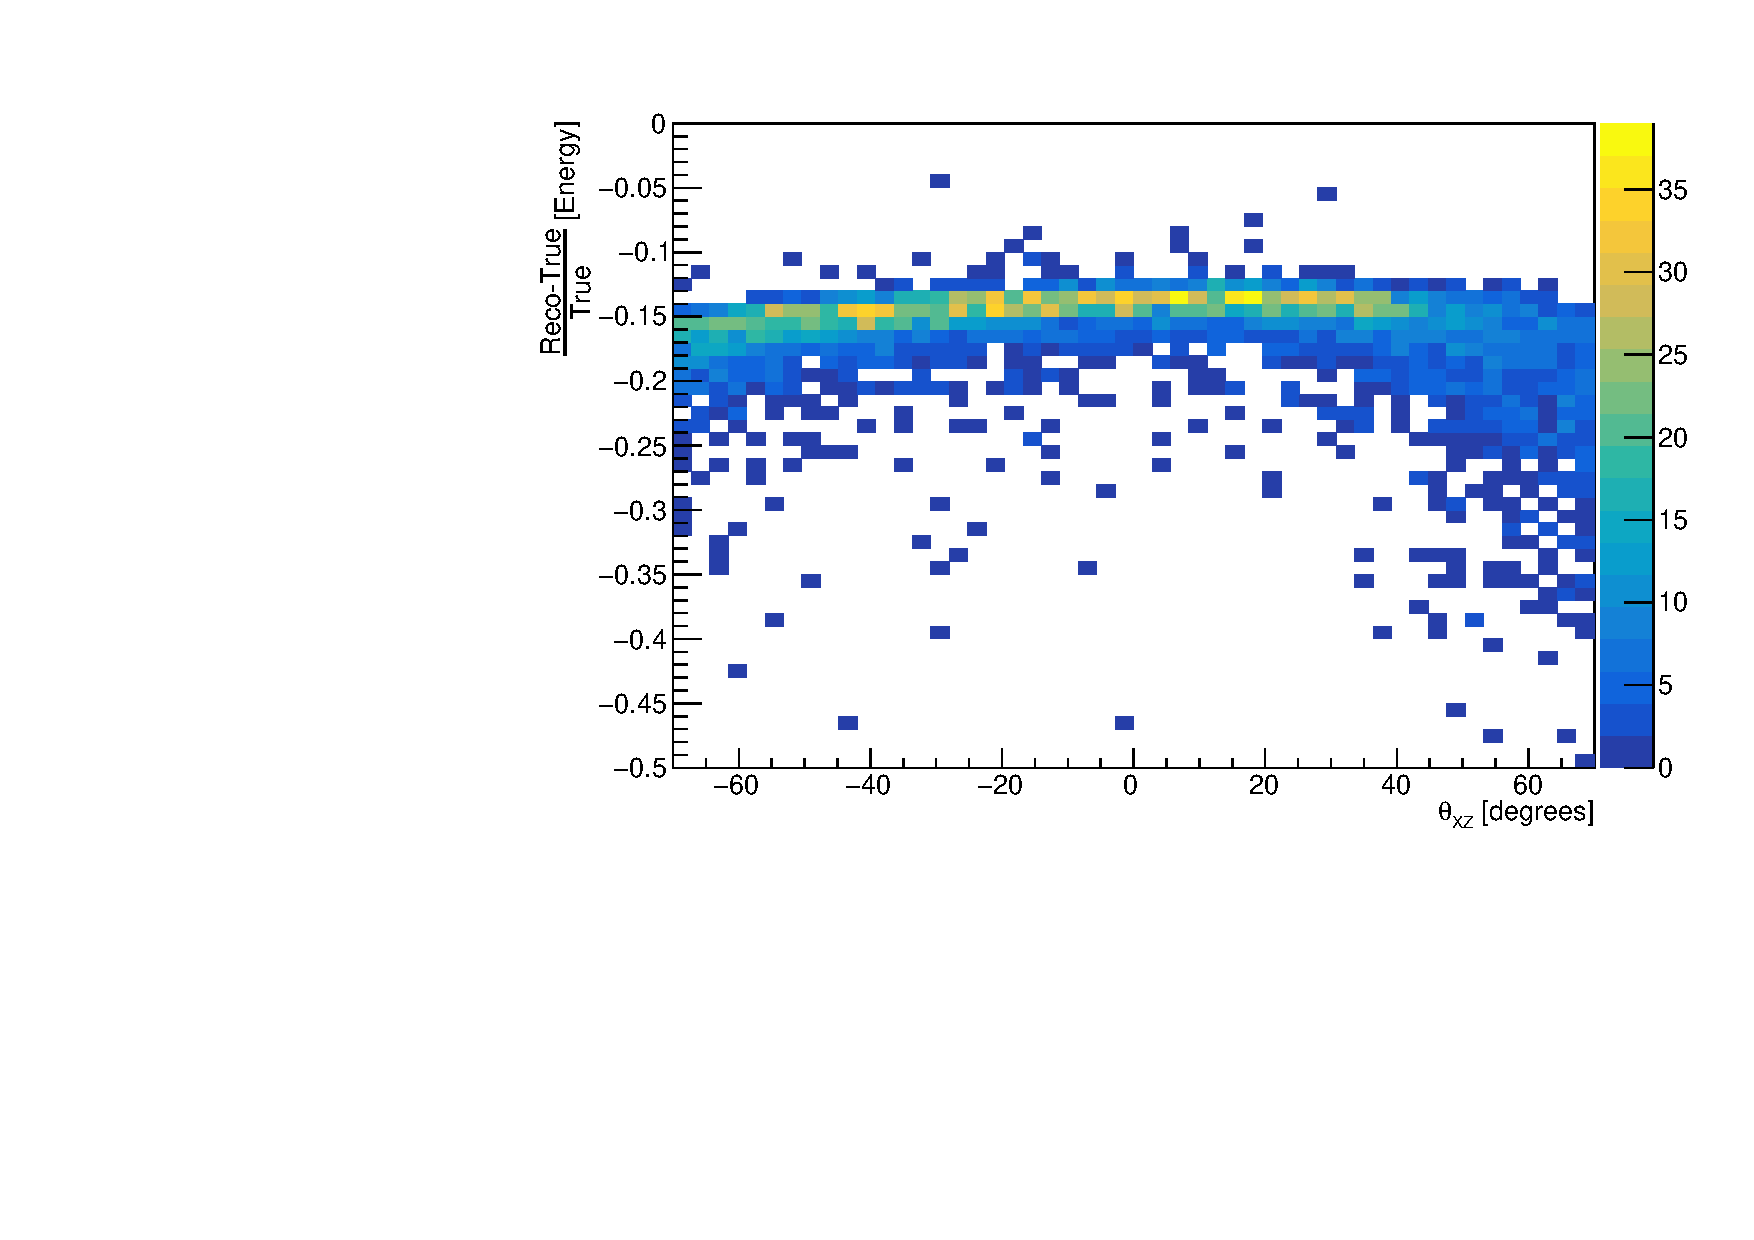
\includegraphics[width = 0.49\textwidth]{figures-chap4/frac_res_vs_thetaXZ_showeringE_cheating_electron_vertex_plane2_cut.pdf}
    \caption[Shower energy reconstruction performance as a function of $\theta_{xz}$.]{Shower energy reconstruction performance as a function of $\theta_{xz}$. Left: true energy is calculated from the hits. Right: true energy is the energy of the showering electron.}
    \label{fig:reconstruction_as_a_function_of_angle}
\end{figure}



\subsection{Performance as a Function of Energy}
The electromagnetic showers produced in \gls{sbnd} from the \gls{bnb} are expected to have energies up to around a GeV. 
Since the energy range is relatively broad, the reconstruction performance is evaluated as a function of the energy in order to confirm that the reconstruction methods work sufficiently well for all energies. As was the case for the angular dependence, the performance as a function of energy is expected to be similar across the different reconstruction methods with the only difference being in the actual reconstruction performance. 

\newpage
Other Validation stuff to do?
\begin{itemize}
    \item Use photon sample?
    \item validate for each individual plane and then best plane?
    \item Look at all showers in an event and compare with total showering energy. 
\end{itemize}


\section{Summary + outstanding issues etc}

Why getting dE/dx is hard (page 17).
Using muons as calibration
Energy bias corrections
https://inspirehep.net/files/f10063871db4836eb6ad935fcf761e7d

Energy Reco - Things to include.

\begin{itemize}
	\item Motivation (why do we care?)
	\item Explain choices - use vertex sample because it helps pandora. Only considering largest shower (most hits) from each event. 
	\item Overview of the very first method that was being used. Use muons to generate lookup curve. Get linear relationship between deposited charge and energy. Plagiarise Dom's thesis on this..  
	\item Change method so we convert the deposited charge to number of electrons and then convert the number of electrons to energy using the appropriate calibration/scale factors. Apply correction for electron lifetime as before and also correct for recombination. Previously recombination correction was 'baked' into the look-up curve. No way to correct for it directly - whenever we would change the \textit{physics} we would need to regenerate the look-up curve. With this method it's possible to tweak the recombination correction directly. 
	\item Not straight forward to calculate the recombination directly - let's use and average value for all showers - explain recombination study. 
	\item Consider SCE - explain what SC is.
	\item How do we account for SCE? Get map of the E-field in the detector (not uniform because of SC). Using the nominal value of the recombination and E-field, calculate a nominal dE/dx (not straightforward to calculate directly) which we assume remains constant. Can now use the Modified Box model to weak the recombination correction by feeding the local E-field (which depends on the location in the detector) back into the modified box model. Finally, find the (charge weighted) centre of the shower using the space points and use the local E-field at this point to calculate the recombination factor at this location. 
	\item No reason we can't do a per-hit analysis. Redo everything as before for each individual hit and then sum to get the energy of the shower. Should give better results since the recombination correction is more accurate now. 
	\item We have the ability to attempt to correct for the SCE as mentioned, but are limited by not knowing the dE/dx. So correcting the SCE without this caveat becomes tricky.. Try a new approach developed by ArgoNeuT - use the ESTAR database. The ESTAR database gives us the stopping power of (dE/dx) of electrons in various materials (including lAr) in a range of energies and is based partly from data. Combining this with the modified box recombination model, we can again create a lookup curve of energy vs deposited charge with the recombination correction baked in. Since the modified box model depends on the E-Field, we can treat this as a variable and create a 3D lookup curve of energy vs E-Field vs deposited charge which will allow us to correct for SC. 
	\item \textit{True} energy debacle.. We have the true energy of the showering particle and the true energy of all the hits in a given shower. Originally we used the true energy of the showering particle for comparison (in hindsight this seems like a stupid idea..) and the kGeVtoElectrons method clearly outperformed ESTAR. Swapping to the true hit energies, ESTAR does better. What was happening (i think) is that kGeVToElectrons over estimates the hit energies, so when comparing with the true showering particle this method give a better result because we're papering over the cracks due to the pattern recognition and hit inefficiencies. ESATR method gives a better result for individual hit energies so highlights the failing of the patter rec and hit inefficiencies when comparing with the showering particle. 
	\item Why some results are shit.. Pandora pattern recognition (clustering) is far from perfect - can use Pandora in cheating mode to overcome this. There are hit inefficiencies i.e. hit reconstruction isn't perfect - haven't ever \textit{cheated} this, dunno if it's an option. The actual impact from SC is pretty minimal but it also impacts Pandora's pattern recognition. This can a have a big impact - what Pandora initially recognised as one big shower may be interpreted as 2+ smaller showers after applying SC (and vice-versa). Also, an object classified as a shower may instead be classified as a track after applying SC. Since we're only considering the largest shower for each event, this effects mean SC can appear to have a impact. 
\end{itemize}
